\documentclass[10pt,twocolumn]{article}
\usepackage[utf8]{inputenc}
\usepackage[french]{babel}
\usepackage[T1]{fontenc}
\usepackage{amsmath}
\usepackage{amsfonts}
\usepackage{amssymb}
\usepackage{layout}
%\usepackage{setspace}
\usepackage{times}
\usepackage{graphicx}
\usepackage{wrapfig}
\usepackage{layout}

\usepackage[top=2cm, bottom=2cm, left=1cm, right=1cm]{geometry}
\author{jd}

\begin{document}
%\layout


\section{toto}

Un paragraphe\footnote{mon pargraphe}.Un paragraphe.Un paragraphe.Un paragraphe.Un paragraphe.Un paragraphe.Un paragraphe.Un paragraphe.Un paragraphe.Un paragraphe.Un paragraphe.Un paragraphe.Un paragraphe.Un paragraphe.Un paragraphe.Un paragraphe.Un paragraphe.Un paragraphe.Un paragraphe.Un \begin{tiny}
paragraphe.Un paragraphe.Un paragraphe.Un paragraphe.Un paragraphe.Un paragraphe.Un paragraphe.Un paragraphe.Un paragraphe.Un paragraphe.Un paragraphe.Un paragraphe.Un paragraphe.Un paragraphe.Un paragraphe.Un paragraphe.Un paragraphe.Un paragraphe.Un paragraphe.Un paragraphe.
\end{tiny}

\begin{figure}[ht]
\begin{center}
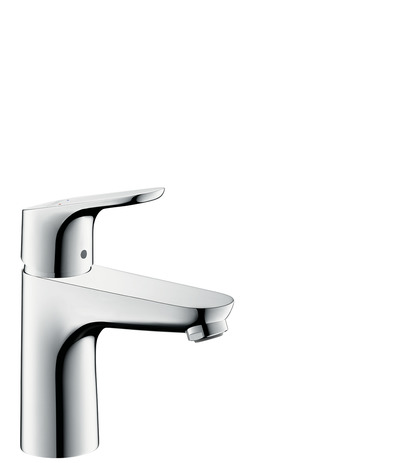
\includegraphics[height=200px]{images/mitigeur_hansgrohe.jpg} 
\caption{Poulpy est88 multicolore}

\label{fstsdf} 
\end{center}
\end{figure}


Un paragraphe.Un paragraphe.Un paragraphe.Un paragraphe.Un paragraphe.Un paragraphe.Un paragraphe.Un paragraphe.Un paragraphe.Un paragraphe.Un paragraphe.Un paragraphe.Un paragraphe.Un paragraphe.Un paragraphe.Un paragraphe.Un paragraph figurel~\ref{Tux} e.


\section{titi}
Un paragraphe.Un paragraphe.Un paragraphe.Un paragraphe.Un paragraphe.Un paragraphe.Un paragraphe.Un paragraphe.Un paragraphe.Un paragraphe.Un paragraphe.Un 

\begin{figure}[ht]
\begin{center}
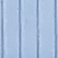
\includegraphics{images/favicon.png} 
\caption{Poulpy est88 multicolore}4545454
\label{Tux}
\end{center}
\end{figure}


\begin{wrapfigure}[9]{r}{4cm}
\begin{center}

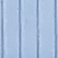
\includegraphics[width=3cm]{images/favicon.png}
\caption{mon favicon}

\end{center}
\end{wrapfigure}

Un paragra phe.Un paragraphe.Un paragraphe.Un paragraphe.U n paragraphe.Un parag raphe.Un paragraphe.Un parag raphe.Un paragra phe.Un paragraphe.Un paragr aphe.Un paragraphe.Un paragraphe.Un paragraphe.Un paragraphe.Un paragraphe.Un paragraphe.Un parag raphe.Un paragraphe.Un paragraphe.Un paragraphe.Un paragraphe.Un paragraphe.Un paragraphe.Un paragraphe.Un paragraphe.Un paragraphe.Un paragraphe.Un 

paragraphe.Un paragraphe.Un paragraphe.Un paragraphe.Un paragraphe.Un paragraphe.Un paragraphe.Un paragraphe.Un paragraphe.Un paragraphe.Un paragraphe.
{\fontfamily{pcr}\selectfont mon bout de texte}

un canard\footnote{bestiole qui fait coin}
un ornithorynque\footnote{bestiole qui fait rire}
un ours\footnote{bestiole qui fait mal}


\end{document}